\scanpage{55}
% top, lines 1–4
A) \uline{2 inv.}\quad \deleted{Alors $f(\lambda s_0+\mu\unsure{\widetilde{o}|\widetilde{\sigma}|\widetilde{c}})=0$ $\forall\lambda,\mu$ \inserted{$g(\lambda,\mu)$ est ident} sss \unsure{$\sigma'$|$\sigma$}} Alors, indépendamment de la parité de $n$, on peut écrire $g(\lambda,\mu)=-\sigma\mu(\lambda+\frac{\rho}{2}\mu)$, et les équivalences décrites dans 1°) sont valables, avec $\rho'$ remplacé par $\rho/2$.

% upper left, line 5
\deleted{b) $S$ de car. 2}

% upper, lines 5–8
Les solutions de $g(\lambda,\mu)=0$, avec $\mu$ inv, sont multiples de $(-\frac{\rho}{2},1)$ et correspondent à $-\frac{\rho}{2}s_0+\widetilde{o}$ ou encore \deleted{$-\unsure{\rho/2}s_0+o$} (si $\rho$ inv. i.e. $\underline a$ défini)
\[
-s_0+2\frac{\widetilde{o}^{\unsure{+}}}{\rho}=o'-\beta_0=\underline a\,s_0
\]

% upper middle, lines 9–10
B) $2\cdot1_S=0$ i.e. $S$ de car. 2. On trouve alors \deleted{$f(\lambda s_0+\mu\widetilde{o})$}

% upper middle, lines 10–12
\[
\begin{aligned}
g(\lambda,\mu)&=f(\lambda s_0+\mu\widetilde{o})=\unsure{+|-|\deleted{-}}(\sigma'\rho')\mu^2\\
&\text{c'est }\equiv0\text{ sss }\sigma'\rho'=0\\
&\text{c'est }\ne0\text{ en tte fibre sss }\sigma'\rho'\text{ inv. i.e. }\sigma'\text{ et }\text{\uuline{$\rho'$}}\text{ inv.}
\end{aligned}
\]

% middle left
\margin{$\underline a\,x=x+o'=x$ \deleted{$f(x+o')=f(x)+f(o')+\langle x,\psi(o')\rangle$} car comme $\rho=\rho'$, \unsure{$s$}}

% middle, lines 13–16
i.e. $\sigma'$ inv et $\underline a$ \deleted{\unsure{$E$|$\mathcal E$}} défini (c'est le cas si $(E,V,f)$ birégulier). \deleted{\unsure{Il}} Ceci signifie aussi $D_0\not\subset Q_X$ en ttes fibres, et implique que $D_0$ est tangente à $Q_X$

% middle, horizontal rules
\figure{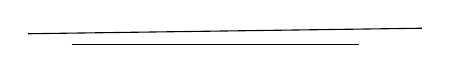
\begin{tikzpicture}\draw (0,0)--(5,.07);\draw (.55,-.14)--(4.2,-.14);\end{tikzpicture}}

% lower, lines 17–25, crossed by two long strokes
\deleted{Supposons $n$ pair, $n=2m$. On s'intéresse aux systèmes $(X,\tau_*=(\tau_i)_{0\le i\le n},s_0)$ \deleted{\unsure{tels}} non dégénérés, et tels que $\sigma\ (= \sigma')$ soit inv. [Si on suppose déjà les $\beta_i$ (i.e. $0\le i\le n-1$) inv, celà signifie $f_E$ lisse.] \deleted{Ceci définit donc} Ceci définit donc $(X,\underset{\text{\unsure{hyperquadrique|hyp. quadrique}}}{Q_X},\tau_*^X)$, où maintenant les $\tau_*$ \inserted{$(0\le i\le n)$} sont des autom. \deleted{de} involutifs de $(X,Q_X)$. Considérons la restriction :}

% lower, last line
\[
(C,Q_C,\tau_*^C)\quad -
\]

% foot, left
% archive sheet number: 54

